\subsubsection{\stid{2.10} PROTEAS | TAU Performance System}\label{subsubsect:tau}

\paragraph{Overview} 
The TAU Performance System is a versatile profiling and tracing toolkit that supports performance instrumentation, measurement, and analysis. It is a robust, portable, and scalable performance tool for use in parallel programs and systems over several technology generations. It is a ubiquitous performance tool suite for shared-memory and message-passing parallel applications written in C++, C, Fortran, Java, Python, UPC, and Chapel. In the PROTEAS project, TAU is being extended to support compiler-based instrumentation for the LLVM C, C++, and Fortran compilers using higher-level intermediate language representation. TAU is also targeting support for performance evaluation of directive based compilation solutions using OpenARC and it will support comprehensive performance evaluation of NVM based HPC systems.  Through these and other efforts, our objective to better support parallel runtime systems such as OpenMP, OpenACC, Kokkos, ROCm, and CUDA in TAU. Figure~\ref{figure:tau} gives an example of using TAU's parallel profile analysis tool, ParaProf.

\paragraph{Key Challenges} 
Scalable Heterogeneous Computing (SHC) platforms are gaining popularity, but it is becoming more and more complex to program these systems effectively and to evaluate their performance at scale. Performance engineering of applications must take into account multi-layered language and runtime systems, while mapping low-level actions to high-level programming abstractions.  Runtime systems such as Kokkos can shield the complexities of programming SHC systems from the programmers, but pose challenges to performance evaluation tools.  Better integration of performance technology is required.  Exposing parallelism to compilers using higher level constructs in the intermediate language provides additional opportunities for instrumentation and mapping of performance data.  It also makes possible developing new capabilities for observing multiple layers of memory hierarchy and I/O subsystems, especially for NVM-based HPC systems. 

\paragraph{Solution Strategy} Compilers and runtime systems can expose several opportunities for performance instrumentation tools such as TAU.  For instance, using the OpenACC profiling interface, TAU can tap into a wealth of information during kernel execution on accelerators as well measure data transfers between the host and devices. This can highlight when and where these data transfers occur and how long they last.  By implementing compiler-based instrumentation of LLVM compilers with TAU, it is possible to how the precise exclusive and inclusive duration of routines for programs written in C, C++, and Fortran.  Furthermore, we an take advantage of the Kokkos profiling interface to help map lower level performance data to higher level Kokkos constructs that are relevant to programmers. The instrumentation at the runtime system level can be achieved by transparently injecting the TAU Dynamic Shared Object (DSO) in the address space of the executing application. This requires no modification to the application source code or the executable. 

\begin{figure}[htb]
\centering
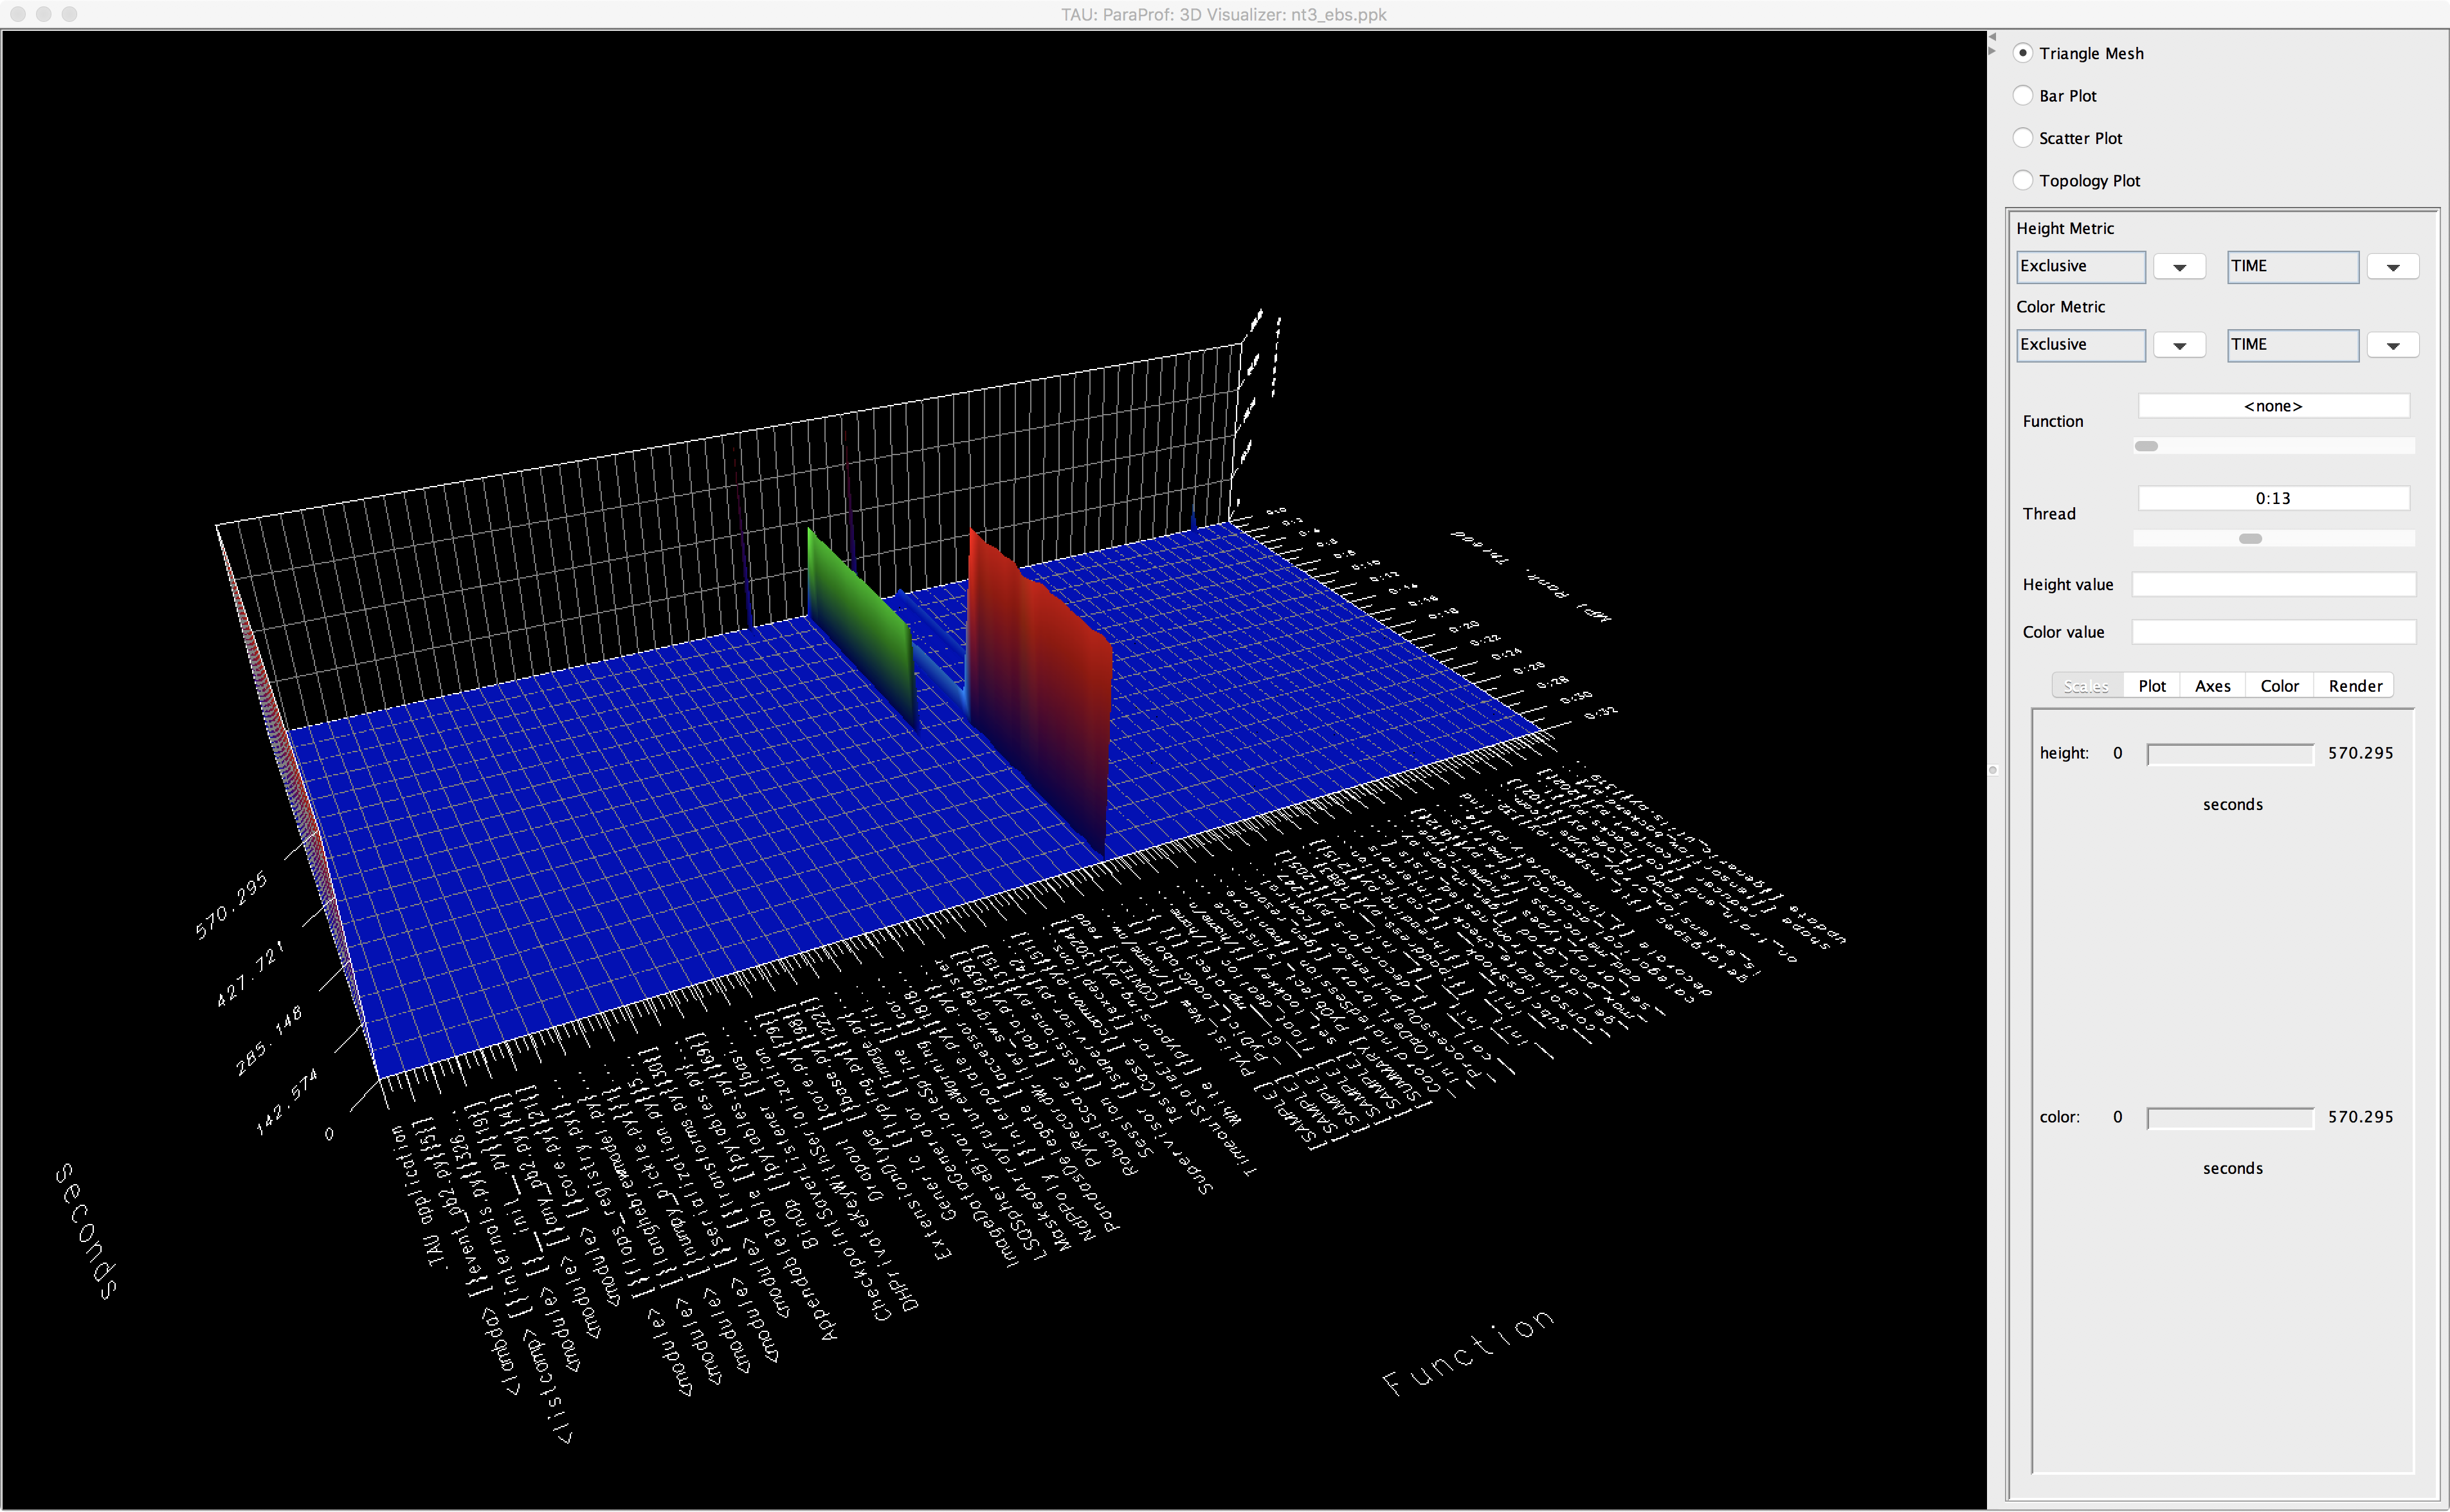
\includegraphics[width=6in]{projects/2.3.2-Tools/2.3.2.10-PROTEAS-YTUNE/tau-3d-candle}
\caption{
  TAU's ParaProf profile browser shows the parallel performance of the CANDLE application, where half the threads are engaged in one activity (\texttt{pthread\_cond\_wait}) while the other half is engaged in some other activity (\texttt{Eigen::internal::gebp\_kernel}).
}
\label{figure:tau}
\end{figure}

\paragraph{Recent Progress}
\begin{enumerate}
\item \textbf{CANDLE} Extended TAU to enhance performance evaluation of multii-threaded Python3 and CUDA and applied it to evaluate the performance of the CANDLE ECP Benchmarks.

\item \textbf{Improved CUDA and OpenMP support} Added support for newer GPUs and enhancements to the CUPTI profiling interface in TAU, including multithreaded kernel launch support.  Further updated the OpenMP Tools Interface support in TAU, to support the evolving 5.0 standard. 

\item \textbf{NVM Measurement} Updated support for PAPI and LIKWID hardware counter library, which exposes memory hierarchy counters to TAU.

\item \textbf{LLVM Instrumentation} Per-function selective instrumentation support for compiler-based instrumentation was implemented in TAU, using a TAU LLVM plugin.

\item \textbf{AMReX} TAU OpenACC measurement was demonstrated on the AMReX library.

\item \textbf{CODAR} TAU integrated measurement of ADIOS 1.13 using a callback mechanism, and runtime performance data aggregation and monitoring of a coupled fusion simulation using the Scalable Observation System (SOS).
\end{enumerate}

\paragraph{Next Steps}
\begin{enumerate}
\item \textbf{NVM instrumentation} 
Design and implement support for supporting deep memory hierarchies in TAU for supporting MCDRAM based systems. 

\item \textbf{NVM Measurement} 
Comprehensive profiling and tracing support for NVM architectures.

\item \textbf{PHIRE} 
Improved LLVM IR-based instrumentation using PHIRE.

\item \textbf{Outreach}
Continued outreach activities to demonstrate comprehensive performance evaluation support in TAU for OpenARC, LLVM, CUDA, Kokkos, ROCm, and NVM based programming frameworks for SHC platforms. 
\end{enumerate}
